\chapter{Resultados}
\label{cap:Resultados}

En este capítulo se expondrán los resultados obtenidos a lo largo del desarrollo del proyecto, tras aplicar la metodología definida en el Capítulo \ref{cap:Metodologia}. De esta manera, se detallará en primer lugar una visión general del proyecto, compuesto por la planificación de las versiones, sus objetivos y el contexto en el que se enmarcan. Además, se desarrollará en este capítulo los sprints que se han llevado a cabo, junto con las funcionalidades que se han incluido en cada una de las versiones.

\section{Visión Global}
\label{sec:VisionGlobal}

Como se indicó anteriormente el OP de este proyecto consiste en el diseño y desarrollo de un JS de escritorio, cuyo aprovechamiento sirva para la enseñanza y el apoyo hacia aquellos usuarios que desean aprender conocimientos sobre el nuevo modelo de desarrollar software llamado DGS y en especial, como se lleva a cabo la labor de gestionar proyectos de estas características, utilizando técnicas de gamificación e inteligencia artificial.

\textbf{Grupo Objetivo}

El JS obtenido como resultado estará destinado en especial a estudiantes de ingeniería de software que desean aprender conocimientos sobre como se lleva a cabo el desarrollo de software en proyectos DGS, además de experimentar como llevar a cabo la gestión de este tipo de proyectos. Por otro lado, también estará dirigido a aquellos profesionales de la ingeniería del software que deseen ampliar sus conocimientos en otros modelos de desarrollar software, en especial con esta nueva tendencia, y así estar entrenados ante situaciones que puedan ocurrir en este tipo de proyectos y poder trabajar en un futuro en un entorno real.

\textbf{Necesidades}

La aparición de este nuevo modelo de desarrollo y la importancia que está tomando en los últimos años en el mundo laboral, hace necesaria la existencia de una buena educación y enseñanza de los aspectos y conceptos que lo engloban tanto en el ámbito estudiantil como en el laboral. Incluso, se añade la manifestación del fracaso de un gran número de proyectos con entornos globales debido, en especial mediada a su desconocimiento por parte de los miembros y a la difícil gestión que conlleva esta clase de proyectos, por lo que se hace necesario un entrenamiento previo.

\textbf{Producto}

Con este proyecto de TFG, se pretende obtener como resultado un JS de escritorio que permita a los jugadores jugar diferentes partidas, en donde el jugador (con el rol de jefe de proyecto) deberá gestionar un proyecto DGS ficticio, en el cual aparecerán múltiples situaciones o contratiempos que puedan ocurrir en un ambiente de estas características, las cuales deberán ser solventadas por el jugador.

\textbf{Beneficios}

Los beneficios que conlleva la utilización de esta herramienta consisten en el aprendizaje de un nuevo modelo de desarrollo de software, el cual está tomando cada vez más importancia y puede ser desconocido por un gran número de personas en la actualidad. Además, permite entrenarse en un escenario virtual conociéndose así las situaciones que puedan darse en un proyecto real de estas características, y poder afrontar con éxito la gestión del mismo.

El desarrollo del proyecto se ha dividido en tres versiones diferentes, las cuales serán definidas a continuación:

\begin{itemize}
	\item \textbf{Versión 1.} Esta primera versión se corresponderá con la redacción y definición de los requisitos iniciales del futuro JS. Además, se diseñaran los bocetos de las diferentes ventanas y vistas que poseerá la aplicación mediante la plataforma Balsamiq Mockup. Por otro lado, se llevará a cabo el estudio y aprendizaje de la herramienta para el desarrollo de videojuegos, Unity.
	\item \textbf{Versión 2.} Esta versión intermedia se centrará en el diseño de las diferentes interfaces gráficas de usuario de las cuales estará compuesta el juego, junto con el desarrollo del sistema para llevar a cabo una partida. Para ello se implementarán aspectos de gamificación y jugabilidad en el juego. Obtendremos como resultado una aplicación que nos permita jugar diferentes partidas al juego.
	\item \textbf{Versión 3.} Versión final de la aplicación la cual se centrará en la introducción de diferentes aspectos inteligentes sobre el juego, así como un sistema para la asignación de niveles y para poder llevar a cabo una enseñanza acorde con los conocimientos previos de cada usuario.
\end{itemize}

\section{Arquitectura}
\label{sec:Arquitectura}

A continuación, se detallará la arquitectura tecnológica que se ha diseñado para conseguir el desarrollo de Global-Manager, además, de las librerías adicionales utilizadas. 

En la figura \ref{fig:ArquitecturaTecnologica} se puede observar la arquitectura tecnológica del JS.

\begin{figure}[htb]
	\centering
	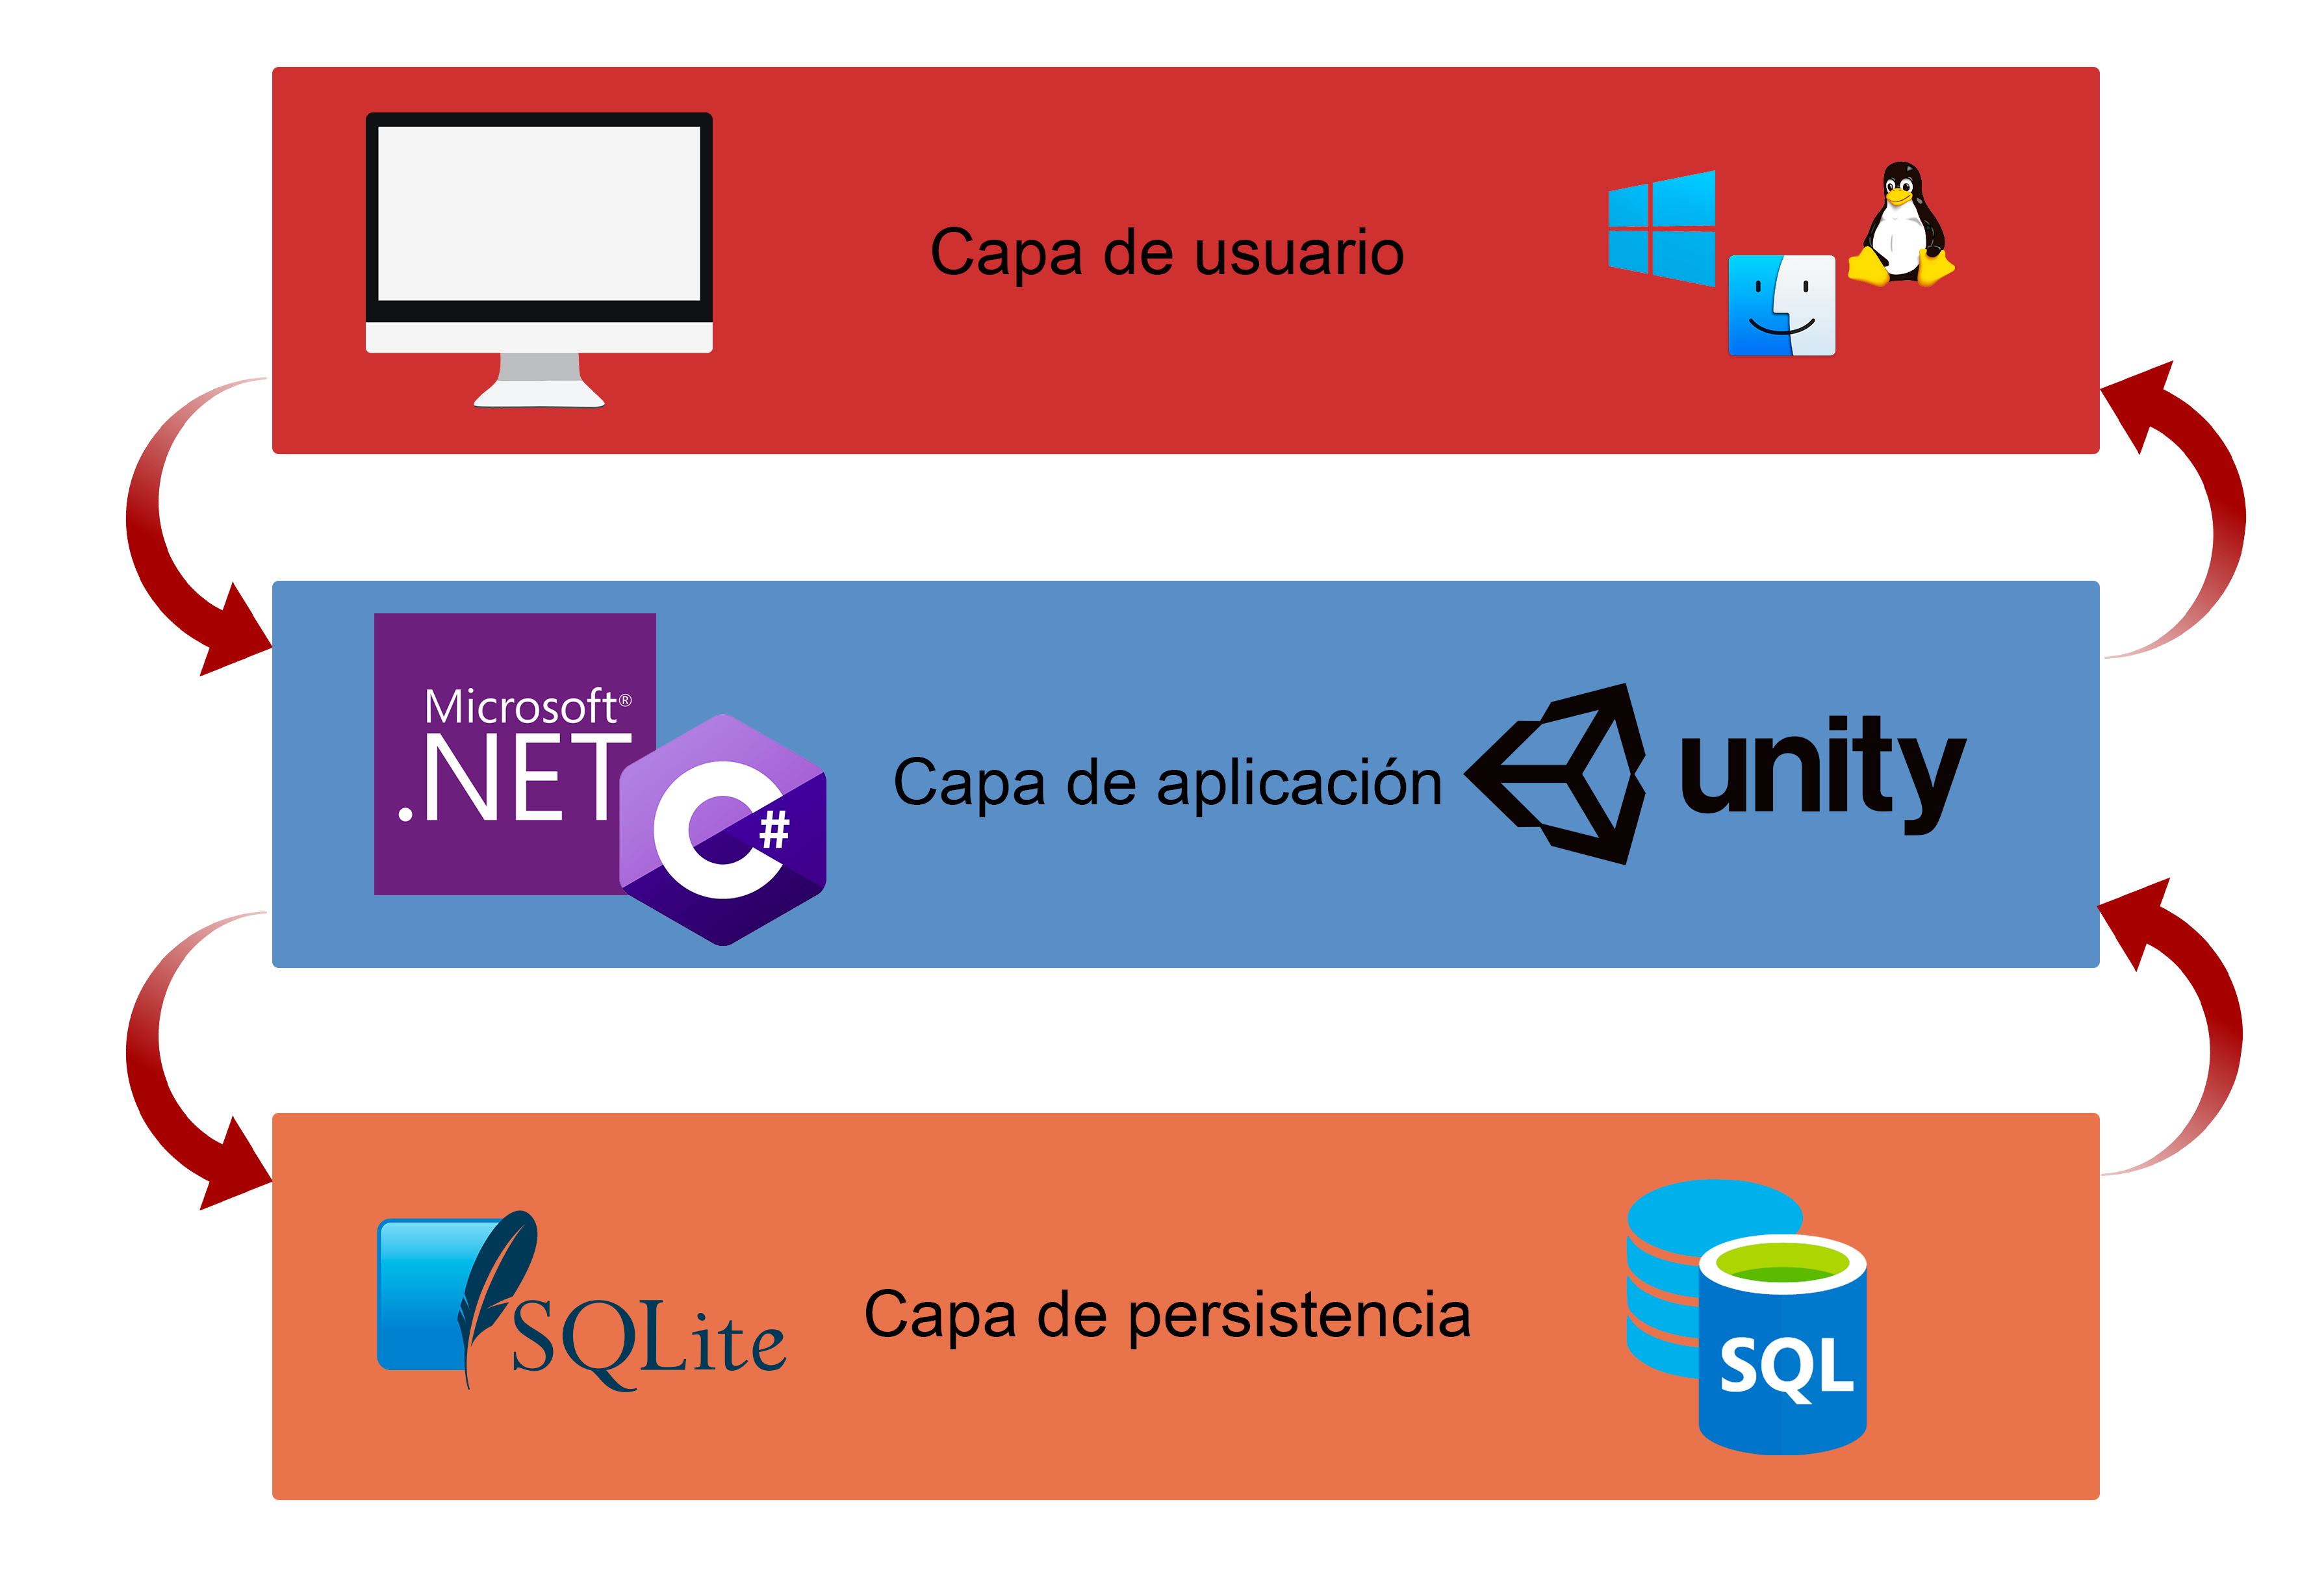
\includegraphics[width=0.95\linewidth]{ArquitecturaTecnologica}
	\caption[Arquitectura tecnológica de Global-Manager]{Arquitectura tecnológica de Global-Manager}
	\label{fig:ArquitecturaTecnologica}
\end{figure}

Dicha arquitectura posee tres capas:

\begin{itemize}
	\item \textbf{Capa de usuario.} Representa el entorno sobre el cual se podrá ejecutar la aplicación. En nuestro caso, el JS consistirá en una aplicación de escritorio, la cual se podrá ejecutar en los sistemas operativos \emph{Windows}, \emph{Linux} y \emph{Mac OS}.
	\item \textbf{Capa de aplicación.} Consiste en la capa que hace referencia al JS, el cual consistirá en un proyecto \emph{.NET Framework}, en el cual se utiliza el motor de videojuegos y físicas, \emph{Unity} junto con diferentes \emph{scripts} escritos en el lenguaje de programación C\#.  
	\item \textbf{Capa de persistencia.} Esta última capa hace referencia a la base de datos o modelo de datos, donde se almacenará toda la información relevante tanto de la aplicación como de los usuarios. Para ello, se ha optado por utilizar como motor de base de datos \emph{SQLite}, de esta manera existirá una base de datos SQLite en local y se llevará a cabo el intercambio de información mediante sentencias SQL.
\end{itemize}